\documentclass{article}

% if you need to pass options to natbib, use, e.g.:
% \PassOptionsToPackage{numbers, compress}{natbib}
% before loading nips_2016
%
% to avoid loading the natbib package, add option nonatbib:
% \usepackage[nonatbib]{nips_2016}

\usepackage[final]{nips_2016}

% to compile a camera-ready version, add the [final] option, e.g.:
% \usepackage[final]{nips_2016}

\usepackage[utf8]{inputenc} % allow utf-8 input
\usepackage[T1]{fontenc}    % use 8-bit T1 fonts
\usepackage{hyperref}       % hyperlinks
\usepackage{url}            % simple URL typesetting
\usepackage{booktabs}       % professional-quality tables
\usepackage{amsfonts}       % blackboard math symbols
\usepackage{nicefrac}       % compact symbols for 1/2, etc.
\usepackage{microtype}      % microtypography
\usepackage{amsmath}        % used for armgmind
\usepackage{listings}       % Required for insertion of code
\usepackage{parcolumns}     % Required for 2-column listings.
\usepackage{float}          %Required for fixing position of figures.
\usepackage{hyperref}       %Required for hyperlink to github site.
\usepackage{graphicx}       % Required to insert images

\title{Imputing Missing Data and Feature Selection via Penalized Matrix Decomposition}

%CUSTOMIZE INDENTS:
\newcommand{\myindent}{\hspace*{1cm}}
\setlength{\parindent}{0pt}

%ARGMIN:
\DeclareMathOperator*{\argmin}{argmin}

% The \author macro works with any number of authors. There are two
% commands used to separate the names and addresses of multiple
% authors: \And and \AND.
%
% Using \And between authors leaves it to LaTeX to determine where to
% break the lines. Using \AND forces a line break at that point. So,
% if LaTeX puts 3 of 4 authors names on the first line, and the last
% on the second line, try using \AND instead of \And before the third
% author name.

\author{
  Jennifer Starling \& Jesse Miller\\%\thanks{Use footnote for providing further
    %information about author (webpage, alternative
    %address)---\emph{not} for acknowledging funding agencies.} \\
  Department of Statistics \& Data Science\\
  University of Texas at Austin\\
  %Austin, TX \\
  %\texttt{hippo@cs.cranberry-lemon.edu} \\
  %% examples of more authors
  %% \And
  %% Coauthor \\
  %% Affiliation \\
  %% Address \\
  %% \texttt{email} \\
  %% \AND
  %% Coauthor \\
  %% Affiliation \\
  %% Address \\
  %% \texttt{email} \\
  %% \And
  %% Coauthor \\
  %% Affiliation \\
  %% Address \\
  %% \texttt{email} \\
  %% \And
  %% Coauthor \\
  %% Affiliation \\
  %% Address \\
  %% \texttt{email} \\
}

\begin{document}
% \nipsfinalcopy is no longer used

\maketitle

\begin{abstract}
We compare several methods of imputing values for missing data with continuous and categorical variables in the logistic regression setting.  We apply penalized matrix decomposition to impute missing continuous values and compare the results to two other methods.  We compare two methods for imputing missing categorical values.  We finish by performing variable selection to compare several different models.
\end{abstract}

\section{Introduction}

Regression in the presence of missing data values is a well-studied but still relevant problem.  Many simple proposed solutions exist, including exclusion of observations with one or more missing predictors from the data set, imputing missing values with each predictor's mean value, and others.

The setting for this project is prediction of whether an undergraduate student will pass an introductory Calculus course.  The data is from the fall 2014 and fall 2015 semesters at the University of Texas at Austin (UT), and contains observations for all students who took an in-residence introductory Calculus class (M408C/K/N/R).  Given how many students are required to take Calculus as part of their degree plans, it is important to be able to predict which students are likely to pass.  Among other things, accurate predictions would allow UT to direct students who are likely to fail to remedial material that would help them prepare for Calculus.

Prediction of the binary response Pass/Fail could be handled in many ways (logistic regression, $K$-Means, random forest, etc.), which all perform optimally in the absence of missing values.  We use logistic regression in our analyses.

Predictors are both categorical and quantitative; this project focuses on imputing missing values for continuous predictors.  Continuous predictors include SAT and ACT scores, predicted GPAs, AP test scores, scores from ALEKS (an online system formerly used for placement purposes), and scores from the University of Texas Math Assessment (UTMA), which is the current exam used by the UT Math Department for placement into M408C/K/N/R.  Categorical variables include the schools in which students are enrolled, parental income, parental education levels, first-generation-college status, and what, if any, high school Calculus students have had.

Data in this setting typically contain many missing values.  For example, students commonly take either the SAT or ACT, but usually not both.  Students also rarely take all AP tests.  The data set contains 6,266 observations, 28 continuous predictors, and has about 11\% of the data missing (19,536 missing values out of 175,448 total values).

\section{Related Work}

As described in the Introduction, there are many simple solutions for handling missing continuous data, such as imputation with the mean and excluding observations.  More complex solutions include those proposed by Hastie et al.~in [3].  That paper proposes imputation of missing data via three methods: Singular Value Decomposition, Nearest-Neighbor Imputation, and Imputation Using Regression, which is an Expectation-Maximization-based approach.

A relatively new solution uses properties of penalized matrix decomposition to impute missing values.  This solution is proposed in [7].  This paper describes an algorithm for recovering the rank-$K$ penalized matrix decomposition.

\section{Proposed Work}

We will first summarize the methodology from [7].  Second, we will present two simulated examples to illustrate how the method performs both missing data imputation and variable selection via sparsity.  Third, we will illustrate how the method can be used for feature selection.  Fourth, we impute the missing data values using the penalized matrix decomposition methodology and discuss improvements in a logistic regression model, including comparison to two other methods.  Fifth, we will impute missing categorical values by imputing the mode and compare this to imputing an explicit ``missing'' value.  Last, we will use the best of these methods to build several models and compare them.

\section{Experiment}

\subsection{Method Survey}

We begin by providing a brief survey of the penalized matrix decomposition method.\\

\textbf{Parameter Selections.} The method allows the user to specify a rank (from 1 to the number of predictors) for the decomposition.  For purposes of data imputation, a full rank decomposition is used.  For variable selection, a rank 1 decomposition allows the number of interesting selected variables to decrease towards one.

The method allows the user two specify two penalty terms, $\lambda_U$ and $\lambda_V$.  These penalty terms dictate the sparsity of the $U$ and $V$ matrices in the penalized decomposition.  In the data imputation case, large values of $\lambda$ prove useful, as we are not interested in introducing sparsity in this scenario.  For variable selection, decreasing $\lambda$ progressively results in smaller subsets of variables identified as interesting.  This is discussed in more detail later.\\

\textbf{Rank 1 Penalized Matrix Decomposition.} We first implement the rank 1 sparse matrix factorization algorithm detailed on pages 519--520 of [7]. The R function implementation is {\tt sp.matrix.decomp.rank1()}.

The optimization problem is:
%
%\myindent $\argmin\limits_{u \in R^N, v \in R^p} = ||\bf{X} - d\bf{uv}^T||_F^2 \text{   }$
%subject to
% $||u||_2^2 = 1, ||v||_2^2 = 1,$
% $||u||_1 \leq \lambda_u, ||v||_1 \leq \lambda_v$,\\
%
$$\argmin\limits_{u \in R^N, v \in R^p} = ||\bf{X} - d\bf{uv}^T||_F^2 \mskip12mu\hbox{subject to}\mskip12mu ||u||_2^2 = 1,\ ||v||_2^2 = 1,\ ||u||_1 \leq \lambda_u,\ ||v||_1 \leq \lambda_v,$$
%
where F indicates the squared Frobenius norm of a matrix (sum of squared elements).  This problem is equivalent to:
$$\text{maximize}_{u,v}\bf{ u^TXv}\mskip12mu\hbox{subject to}\mskip12mu ||u||_2^2 = 1,\ ||v||_2^2 = 1,\ ||u||_1 \leq \lambda_u,\ ||v||_1 \leq \lambda_v.$$

The equivalence is proved in the appendix of [7].  The outline of the algorithm is as follows.

\begin{enumerate}
	\item Initialize $v$ to some random vector whose $l_2$ norm equals 1.
	\item Let $u = \frac{S_{\theta_u}(Xv)} {||S_{\theta_u}(Xv)||_2}$
	\item Let $v = \frac{S_{\theta_v}(X^T u)} {||S_{\theta_v}(X^T u)||_2}$
	\item Repeat until convergence is reached.
\end{enumerate}

The convergence criteria is $sum(abs(v.old - v.new)^2 < \epsilon$.  Two technical details:

\begin{itemize}
	\item $S_{\theta_v}(a) = \text{sign}(a)(|a| - \theta_v)_+$ is the same soft-thresholding operator used in the LASSO solution.
	\item $\theta_u$ and $\theta_v$ are found using binary searches within each iteration.\\
\end{itemize}


\textbf{Rank K Penalized Matrix Decomposition.} There is an outline in [7] of a recursive strategy to derive the rank $K$ penalized matrix decomposition.  This recursion relies on repeated use of the rank 1 algorithm. The R function implementation is {\tt sparse.matrix.decomp.rankk()}.

The outline of the algorithm is as follows.

\begin{enumerate}
	\item Initialize $v$ to some random vector where the $l_2$ norm equals 1.
	\item Let $\bf{X^1} = \bf{X}$.
	\item For $k \in {1,\dots,K}$:
	\begin{enumerate}
		\item Find $\bf{u_k}, \bf{v_k}$ and $d_k$ by using the rank 1 algorithm with input $\bf{X^K}$.
		\item $\bf{X^{K+1}} = \bf{X^K} - d_k \bf{u_k x_k^T}$\\
	\end{enumerate}
\end{enumerate}

\textbf{Missing Data Method.} It is noted in [7] that the algorithm works even when there are missing observations; the missing elements of a matrix $X$ can be excluded from all computations, and so the algorithm can be used to impute missing values.  The algorithm is essentially identical to the rank $K$ method above.  \\

The algorithm is as follows. The set of indices where $X$ has nonmissing values is denoted by $C$.
$$
	\text{maximize}_{u,v} \sum_{(i,j) \in C} X_{ij}u_i v_j\mskip12mu\hbox{subject to}\mskip12mu ||u||_2^2 = 1,\ ||v||_2^2 = 1,\ ||u||_1 \leq \lambda_u,\ ||v||_1 \leq \lambda_v.
$$

\subsection{Example: Illustrating Missing Data Imputation}

This example illustrates using penalized matrix decomposition to impute missing data.  We generate a small ($5\times4$) $X$ matrix of random values.  Then 50\% of these values are randomly set to NA.  The first matrix is the original, and the second matrix is imputed using the penalized matrix decomposition.  The $\lambda$ penalties were set to a large value (ten) in this case, as sparsity is not a desired feature.

\noindent\begin{minipage}{.48\textwidth}
\begin{lstlisting}[caption=Original Matrix,frame=tlrb,basicstyle=\tiny]
     -0.371  -0.869   NA  -0.262
     -0.566  -0.317   NA      NA
         NA   0.022   NA      NA
      0.245  -1.372   NA   0.562
     -0.409      NA   NA      NA
\end{lstlisting}
\end{minipage}\hfill
\begin{minipage}{.48\textwidth}
\begin{lstlisting}[caption=Imputed Matrix,frame=tlrb,basicstyle=\tiny]{Name}
     -0.371  -0.869  -0.244  -0.262
     -0.566  -0.317  -1.326  -0.141
     -0.093   0.022   0.937  -0.098
      0.245  -1.372   1.131   0.562
     -0.409  -0.145  -0.907   0.973
\end{lstlisting}
\end{minipage}

\subsection{Example: Illustrating Feature Selection}

Decreasing the $\lambda$ penalties increases sparsity, effectively selecting a limited number of non-zero elements of $U$ and $V$, leading to a reconstructed $X$ matrix, where $X = U*D*t(V)$, with a limited number of columns containing non-zero elements.

This example uses another toy ($5\times4$) $X$ matrix, this time with no missing values.  It is noted in [7] that to obtain equal levels of sparsity in $U$ and $V$, set a constant $c$, and let $\lambda_U = c\sqrt{n}$ where $n = \text{nrow}(X)$, and let $\lambda_V = c\sqrt{p}$ where $p = \text{ncol}(X)$.  In this example, we used values of $c$ in $\{1.0, 0.8, 0.6, 0.4, 0.2\}$.

This table shows the number of columns in the reconstructed $X = U*D*t(V)$ matrix containing non-zero values.  The number of columns containing at least one non-zero value decreases as $\lambda$ decreases, illustrating the variable selection effect of the $\lambda$ penalties.

\begin{table}[H]
  \caption{Variable Selection by Lambda Penalty}
  \label{sample-table}
  \centering
  \begin{tabular}{cccc}
    \toprule
    $c$   & $\lambda_U$   & $\lambda_V$   &Nonzero $X$ cols \\
    \midrule
    1.0  & 2.236     & 2.0       & 4\\
    0.8  & 1.789     & 1.6       & 4\\
    0.6  & 1.342     & 1.2       & 2\\
    0.4  & 0.894     & 0.8       & 1\\
    0.2  & 0.447     & 0.4       & 1\\
    \bottomrule
  \end{tabular}
\end{table}

\subsection{Missing Data Imputation for Continuous Predictors}

After imputing the continuous predictor data using penalized matrix factorization, a few checks were performed to verify reasonableness.

First, we generated histograms of the raw data for each continuous predictor, with the kernel density estimate of the predictor including imputed data overlaid in blue.  This is a check to ensure that imputing the data is not significantly changing the shape of the distribution of each predictor. The histograms verify that the imputed data is not significantly altering the distribution of any of the predictors.

\begin{figure}[htp!]
  \centering
  \fbox{\rule[-.5cm]{0cm}{0cm}
            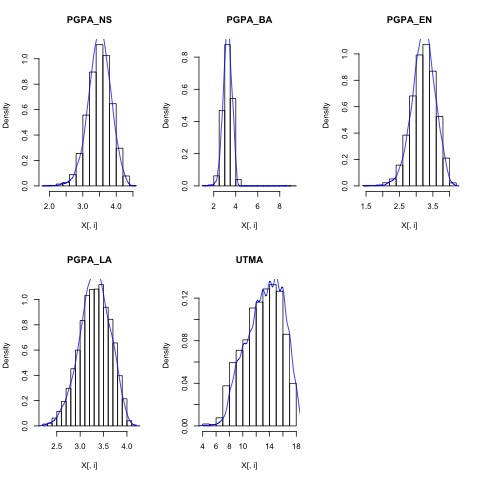
\includegraphics[width=60mm,keepaspectratio]{GPA_hist.jpg}
        \rule[-.5cm]{0cm}{0cm}}
  \caption{Histograms of imputed values for GPA-related predictors \label{fig:1}}
\end{figure}

All imputed variable ranges were checked for reasonableness as well.  Below is an example of checking the ranges of imputed predictors for reasonableness for the SAT-related predictors.

\begin{table}[H]
  \caption{Imputed SAT Range Checks}
  \label{sample-table1}
  \centering
  \begin{tabular}{cccccc}
    \toprule
    \multicolumn{3}{c}{Original} &
    \multicolumn{3}{c}{Imputed}\\

    \cmidrule{1-6}
    SATQ  &SATV &SATTot  & SATQ  &SATV &SATTot\\
    \midrule
     370	& 310	& \phantom{0}770	& 369.88	& 319.83	& \phantom{0}809.77	\\
     800	& 800	& 1600  			& 799.75	& 799.82	& 1599.54			\\
    \bottomrule
  \end{tabular}
\end{table}

Let us now compare the results of performing logistic regression using three methods of imputation.  We split the data into a training set (70\%) and a test set (30\%).  This split was performed for both the original data and the imputed data, yielding two training sets and two test sets.

A logistic regression was performed on the training data with missing values and fit to the test data with missing values.  The test error was 0.31.  A second logistic regression was performed, this time using the training date with imputed values and fit to the test data with imputed values.  The test error was 0.21.

Both of these models were fit using no other model selection techniques; both were fit to all continuous predictors. The imputed data results in a drastic improvement in test error, and the model is now ready to be improved in other ways such as variable selection.

Two other methods of imputing missing data were also compared.  First, imputing missing values using the mean for each predictor resulted in a test error of 0.23.  Second, imputing missing values using singular value decomposition also resulted in a test error of 0.23.  Both methods improved on the original missing data results, but did not yield as much improvement as the penalized matrix decomposition method.

In the remaining sections, we use continuous variables with values imputed using the penalized matrix decomposition method.

\subsection{Missing Data Imputation for Categorical Predictors}

Two methods of imputation of missing categorical values were considered: imputing the mode of each variable, and imputing an explicit ``missing'' value to create an additional category for each variable.  We again used a 70/30 split of the two imputed data sets into two pairs of training and testing sets.  Averaging over 10 splits, we obtained the following test errors for logistic regression models using only categorical variables and models using all variables, with missing continuous values imputed using the matrix method.
\begin{table}[H]
	\caption{Error Rates for Mode Imputation versus ``Missing'' Imputation}
	\label{Categorical Imputation}
	\centering
	\begin{tabular}{lcc}
		\toprule
								& Mode	& Missing	\\
		\midrule
		categorical variables	& 0.257	& 0.247		\\
		all variables			& 0.216	& 0.215		\\
		\bottomrule
	\end{tabular}
\end{table}
In both cases, we can see a slight improvement by adding a ``missing'' category over imputing the mode, although the improvement nearly disappears in the presence of the continuous variables.  In the remaining section, we use categorical variables with a ``missing'' value imputed.



\subsection{Variable Selection}

\underline{Variable Selection via Penalized Matrix Decomposition:}\\

First, the $\lambda$ penalty parameters of the matrix decomposition method were adjusted to explore use of this method as a feature selection tool.  The following $\lambda$ combinations were tested.

\begin{table}[H]
  \caption{Variable Selection via Penalized Matrix Decomposition}
	\label{Penalized Decomp Variable Selection}
	\centering
	\begin{tabular}{ccccc}
		\toprule
					c & $\lambda_U$ & $\lambda_V$ & Predictors Included & Test Error\\
		\midrule
     0.30 &  23.747  & 1.775 &   35  &                  0.21\\
     0.20 &  15.832  & 1.183 &    34  &                  0.23\\
     0.10 &  7.916   & 0.592 &    25  &                  0.23\\
     0.05 &  3.958   & 0.296 &    16  &                  0.23\\
     0.01 &  0.792   & 0.059 &    \phantom{0}6   &                  0.25\\
		\bottomrule
	\end{tabular}
\end{table}

\begin{figure}[!htp]
  \centering
  \fbox{\rule[-.5cm]{0cm}{0cm}
            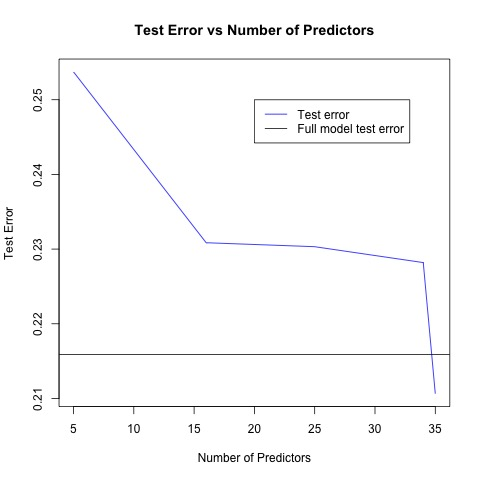
\includegraphics[width=60mm,keepaspectratio]{testerrs.jpg}
        \rule[-.5cm]{0cm}{0cm}}
  \caption{Test Error \label{fig:2}}
\end{figure}
This method was not as successful for variable selection as we had hoped.  The test error rate for the most parsimonious was 0.21, which matched the test error rate when including all continuous predictors.  Additionally, the model with the best test error only eliminated one predictor.  With a full set of 36 predictors, other methods would be perhaps more effective in producing a simpler but more effective model.

The values for $c$, and subsequently the $\lambda$ values, were chosen as described in the method section to impose equal levels of sparsity on the $U$ and $V$ components of the penalized matrix decomposition.  A further area for investigation could be the effectiveness of testing differing levels of sparsity when performing variable selection using the penalties.

After ruling out adjustment of the penalty values as an effective method of variable selection, we proceeded to perform various variable selection techniques on the entire data set, including categorical and continuous predictors together.\\

\underline{General Variable Selection with Continuous and Categorical Predictors:}\\

The following table shows the error rate for several different models, listed in descending order of error rates.  One model was obtained using stepwise selection to determine the variables.  Backward selection was also done, but this resulted in the same model as stepwise selection.  Three others were obtained using penalized matrix decomposition (PMD) to choose from among the continuous variables, as described above.  (The categorical variables in those cases were not considered.)  Several context-important models are also included.  The UTMA is the current placement exam for introductory Calculus at UT, so its performance on its own was tested.  The SAT and ACT tests are very common standardized tests and are often used for admission criteria and placement purposes, so we tested a model that includes the SAT quantitative score and the ACT math score.  The benchmark error rate is the rate using the trivial model that predicts that everyone will pass.  The culled full model includes all predictors except two that are each sums of two other predictors, two with the same entry for all students, and one with no data prior to imputation.
\begin{table}[H]
	\caption{Model Testing, in Descending Order of Error Rates}
	\label{Variable Selection}
	\centering
	\begin{tabular}{lccc}
		\toprule
				& \# of Continuous	& \# of Categorical	\\
		Model	& Predictors		& Predictors	& Error Rate	\\	
		\midrule
		benchmark				& 0		& 0	& 0.2686170	\\
		PMD ($\lambda=0.01$)	& 5		& 0	& 0.2537234	\\
		SATQ \& ACTMath			& 2		& 0	& 0.2430851	\\
		UTMA					& 1		& 0	& 0.2345745	\\
		PMD ($\lambda=0.05$)	& 16	& 0	& 0.2308511	\\
		PMD ($\lambda=0.1$)		& 25	& 0	& 0.2303191	\\
		stepwise selection		& 20	& 2	& 0.2148936	\\
		culled full model		& 31	& 7	& 0.2143617	\\
		\bottomrule
	\end{tabular}
\end{table}





\section{Conclusions and Further Work}

Imputation of continuous variables using the matrix method led to a more accurate logistic regression model than either the use of the original data or the use of imputed mean values.  Imputation of categorical variables using a ``missing'' value led to a slightly more accurate model than did imputation of modes.  Based on what we have seen so far with this data set, though, it will be difficult to lower the error rate below 20\%.

From the perspective of creating a predictive model, this is somewhat disheartening.  From the perspective of a University, though, perhaps this is good: we are not offering a course whose outcome could have been predicted based on pre-college data alone.  We are offering students something new.

That being said, there are still avenues to explore for model improvement.  There are other methods of imputing values for missing continuous variables.  There are also much more sophisticated methods available for dealing with missing categorical data: [2] and [6] discuss the use of latent class models for imputation, [4] discusses a Bayesian method for imputation, and [1] discusses bias correction.  We can also explore classification methods other than logistic regression.


\section{Source Code}

All project documentation and source code is available in the following github repository.\\

\myindent \url{https://github.com/jstarling1/penalized-matrix-decomp}\\

\newpage
\section*{References}
\small

[1] \ Das, U, Maiti, T, and Pradhan, V.\ \ (2010) {\it Bias correction in logistic regression with missing categorical covariates.}  Journal of Statistical Planning and Inference, {\bf 140}: pp 2478–-2485.

[2] \ Gebregziabher, M.~and DeSantis, S.\ \ (2010) {\it Latent class based multiple imputation approach for missing categorical data.}  Journal of Statistical Planning and Inference, {\bf 140}: pp 3252–-3262.

[3] \ Hastie, T, Tibshirani, R, Sherlock, G, Eisen, M, Brown, P, and Botstein, D.\ \ (1999) {\it Imputing Missing Data for Gene Expression Arrays.} Technical Report, Division of Biostatistics, Stanford University.

[4] \ Li, X.\ \ (2009) {\it A Bayesian Approach for Estimating and Replacing Missing Categorical Data.}  ACM Journal of Data and Information Quality, {\bf 1} (1): Article No.~3.

[5] \ Troyanskaya, O, Cantor, M, Sherlock, G, Brown, P, Hastie, T, Tibshirani, R, Botstein, D, and Altman, R.B.\ (2001). {\it Missing value estimation methods for DNA microarrays.} Bioinformatics, {\bf 17} (6), pp 520-–525.

[6] \ Vidotto, D, Vermunt, J, and Kaptein, M.\ \ (2015) {\it Multiple Imputation of Missing Categorical Data using Latent Class Models: State of the Art.}  Psychological Test and Assessment Modeling, {\bf 57} (4): pp 542--576.

[7] \ Witten, D, Tibshirani, R, and Hastie, T.\ \ (2009) {\it A penalized matrix decomposition, with applications to sparse principal components and canonical correlation analysis.} Biostatistics, {\bf 10} (3): pp 515--534.






\end{document}
